\documentclass[conference,a4paper]{IEEEtran}

\usepackage[utf8]{inputenc}
\usepackage[T1]{fontenc}
\usepackage{amsmath,amssymb}
\usepackage{graphicx}
\usepackage{booktabs}
\usepackage[hidelinks,breaklinks]{hyperref}
\usepackage{url}
\usepackage{cite}
\usepackage{multirow}
\usepackage{array}

\begin{document}

\title{Characterization of Lightweight CNN Architectures with INT8 Quantization for Poultry Fecal Disease Detection on Edge Devices}

\author{
\IEEEauthorblockN{Fatih Jawwad Al Mumtaz}
\IEEEauthorblockA{Department of Informatics\\
University of Darussalam Gontor\\
Email: fatihalmumtaz76@student.cs.unida.gontor.ac.id}
\and
\IEEEauthorblockN{Amirul Al Aziz}
\IEEEauthorblockA{Department of Agricultural Industrial Technology\\
University of Darussalam Gontor\\
Email: amirulalaziz57@student.tip.unida.gontor.ac.id}
}

\maketitle

\begin{abstract}
Poultry fecal disease detection with deep learning achieves high accuracy, but prior work largely targets cloud inference with heavy models that are impractical on farms. This paper presents a systematic characterization of three lightweight convolutional neural network architectures---MobileNetV2, ShuffleNetV2, and EfficientNet-B0---for classifying poultry fecal images into four disease categories: Coccidiosis, Salmonellosis, Newcastle Disease, and Healthy. We use the FecalFed leak-free poultry-fecal benchmark~\cite{chi2026} via HuggingFace \texttt{Dianyo/poultry-fecal-fl} (8,770 deduplicated images; publisher splits train=7,016 / test=1,754; derived from Zenodo 4628934 with 6,812 images) and evaluate each model under INT8 dynamic PTQ (ONNX Runtime) on an Intel i5-12400F (200 runs, 10 warmup) and a Raspberry Pi~5 (Cortex-A76, ONNX Runtime 1.29.0, 96 thread/batch configs). All three models exceed 97\% FP32 test accuracy (EfficientNet-B0 98.35\%; MobileNetV2 1.85\,ms, 540.8\,FPS on x86). INT8 increases latency by 6.4--30.1$\times$ on x86 and 1.9--2.8$\times$ on RPi5; on RPi5, INT8 scales by only 1.1--1.2$\times$ (1$\rightarrow$4 threads) versus 2.3$\times$ for FP32, showing limited ARM INT8 parallelization. Accuracy exhibits architecture-dependent sensitivity: MobileNetV2 (+0.23\,pp) and ShuffleNetV2 (+0.06\,pp) are robust, while EfficientNet-B0 collapses from 98.18\% to 35.46\% (62.71\,pp drop, Salmonellosis 0.53\%; Table~\ref{tab:quantacc}) due to squeeze-and-excitation sensitivity. Grad-CAM qualitatively localizes the fecal region for MobileNetV2. Together, the results guide hardware-aware model choice for on-farm deployment.
\end{abstract}

\begin{IEEEkeywords}
deep learning, poultry disease detection, lightweight CNN, quantization, edge computing, Grad-CAM
\end{IEEEkeywords}

\section{Introduction}

Poultry production exceeded USD 70.2 billion in the United States in 2024~\cite{dhungana2025}. Coccidiosis, Salmonellosis, and Newcastle Disease (NCD) cause major losses~\cite{machuve2022}. Fecal image analysis enables noninvasive early detection, but laboratory diagnosis remains inaccessible to many small farms~\cite{tasdelen2025}.

Recent deep learning approaches have achieved high accuracy for poultry fecal disease classification. Dhungana~\textit{et al.}~reported 99.12\% accuracy using EfficientNet-B0~\cite{dhungana2025}, while Tasdelen and Arslan achieved 97.1\% with MobileNetV2~\cite{tasdelen2025}. However, these solutions primarily target cloud-based deployment, leaving a critical gap: \textit{how can these models be efficiently deployed on resource-constrained edge devices at farm level?}

Lightweight CNNs---MobileNetV2~\cite{mobilenetv2}, ShuffleNetV2~\cite{shufflenetv2}, and EfficientNet~\cite{efficientnet}---are candidates for edge deployment because they need fewer operations. INT8 post-training quantization (PTQ) reduces size by using 8-bit weights~\cite{jacob2018}. On CPUs without INT8 acceleration, however, PTQ can increase latency rather than reduce it, as reported in ONNX Runtime community threads\footnote{\url{https://github.com/microsoft/onnxruntime/issues/6732}}\footnote{\url{https://github.com/microsoft/onnxruntime/issues/12854}} and reviews~\cite{maulana2026}.

This paper addresses three research questions: (1) How do lightweight CNN architectures compare for poultry fecal disease classification? (2) What is the quantization sensitivity of each architecture under INT8 PTQ on CPU? (3) What is the accuracy--latency--size trade-off for edge deployment?

The main contributions of this paper are summarized as follows. First, we present a systematic comparison of three lightweight CNNs under INT8 PTQ for poultry fecal disease detection, validated on both x86 and ARM (Raspberry Pi~5) with 96 thread and batch configurations. Second, we measure that INT8 PTQ increases latency by 6--30$\times$ on x86 and 1.9--2.8$\times$ on ARM and show that, on ARM, INT8 throughput scales by only 1.1--1.2$\times$ from 1 to 4 threads versus 2.3$\times$ for FP32. Third, we provide hardware-aware deployment guidelines grounded in cross-platform latency, thread scaling, batch scaling, memory, and trade-off and interpretability analysis.

\section{Related Work}

\subsection{Poultry Disease Detection}
Machuve~\textit{et al.}~introduced the foundational dataset of 6,812 PCR-verified fecal images from Tanzanian poultry farms~\cite{machuve2022}. Subsequent work has applied various deep learning architectures: Dhungana~\textit{et al.}~combined YOLOv11 detection with EfficientNet-B0 classification, achieving 99.12\% accuracy and 25.8\,ms inference~\cite{dhungana2025}. Tasdelen and Arslan benchmarked six architectures, finding MobileNetV2 optimal for both accuracy (97.1\%) and training speed~\cite{tasdelen2025}. Degu and Simegn employed YOLO-V3 for region-of-interest detection followed by ResNet50 classification~\cite{degu2023}. Prior work on this dataset has not compared lightweight models under quantization with trade-off analysis.

\subsection{Lightweight CNN Architectures}
MobileNetV2~\cite{mobilenetv2} utilizes inverted residuals with linear bottlenecks and depthwise separable convolutions, achieving efficient feature extraction with 2.23M parameters in our configuration (3.5M in the original paper). ShuffleNetV2~\cite{shufflenetv2} introduces channel shuffle operations for cross-channel information flow with only 1.26M parameters. EfficientNet~\cite{efficientnet} employs compound scaling to uniformly balance network depth, width, and resolution. Hoang~\textit{et al.}~recently compared seven lightweight architectures for plant disease detection, identifying hybrid designs as optimal for edge deployment~\cite{hoang2026}.

\subsection{Model Quantization}
INT8 quantization reduces model size by representing weights with 8-bit integers~\cite{jacob2018}. While theoretically achieving 4$\times$ compression, ONNX Runtime documentation~\cite{onnxruntime2024} explicitly notes that INT8 without hardware support (VNNI, Tensor Cores) may degrade performance due to quantize/dequantize overhead. Community reports confirm multi-fold slowdown on CPU (see footnotes in the Introduction). The white paper on quantization surveys why PTQ without calibration degrades on depthwise and SE layers~\cite{nagel2021}. Maulana and Ramasamy's systematic review further shows that Quantization-Aware Training (QAT) consistently outperforms PTQ~\cite{maulana2026}.

\section{Methodology}

\subsection{Dataset}
We use the Machuve~\textit{et al.}~dataset~\cite{machuve22} with PCR-verified fecal images from Tanzanian farms, as curated via HuggingFace~\texttt{Dianyo/poultry-fecal-fl}. This is the FecalFed leak-free benchmark~\cite{chi2026}: 8,770 deduplicated unique images across four classes (publisher splits train=7,016 / test=1,754), derived from Zenodo 4628934 (6,812 images: cocci 2,103, healthy 2,057, salmo 2,276, ncd 376) with a 46.89\% duplication rate in public repositories eliminated. The publisher test split (1,754) is used as-is and never re-split; validation (1,402) is a stratified 80/20 carve of the publisher \textit{train} split only (seed 42), giving final 5,614/1,402/1,754 with train+val=7,016 verifiable in \texttt{results/splits\_manifest.json}. Classes are Coccidiosis (30.7\%), Healthy (29.2\%), Salmonella (32.5\%), and Newcastle Disease (8.3\% raw; 5.5\% of Zenodo). NCD is underrepresented; we report per-class FP32 and INT8 accuracy (Table~\ref{tab:quantacc}) as a limitation. Images are resized to 224$\times$224 and normalized with ImageNet mean/std.

\subsection{Model Architectures}
We evaluate three ImageNet~\cite{deng2009}-pretrained lightweight architectures with the classification head replaced for four classes. MobileNetV2~\cite{mobilenetv2} (2.23M parameters, measured) uses inverted residuals with depthwise separable convolutions for efficient local feature extraction. ShuffleNetV2~\cite{shufflenetv2} (1.26M parameters, measured) relies on channel shuffle for cross-channel mixing with few parameters. EfficientNet-B0~\cite{efficientnet} (4.01M parameters, measured) applies compound scaling with squeeze-and-excitation blocks to capture multi-scale features. All models are trained from the same seed (42) with best-checkpoint selection on validation accuracy; single-seed results are reported and multi-seed variance is listed as a limitation.

\subsection{Training Protocol}
All models are trained for 50 epochs using Adam optimizer (learning rate $10^{-4}$, weight decay $10^{-4}$) with cosine annealing schedule. Batch size is 32, input resolution $224 \times 224$. Data augmentation includes random horizontal flip, rotation ($\pm 15^\circ$), and color jitter. Training is performed on an NVIDIA RTX 4060 GPU with 8\,GB VRAM using PyTorch 2.5.1 with CUDA 12.1.

\subsection{Quantization and Benchmarking (x86)}
Models are exported to ONNX and quantized with ONNX Runtime dynamic per-tensor INT8 (CPUExecutionProvider, no calibration dataset; weights quantized to INT8, activations dynamically quantized at runtime). This matches the stock ORT PTQ path and explains the architecture-dependent accuracy drop (including EfficientNet-B0 SE blocks). x86 latency is measured on an Intel i5-12400F CPU (CPUExecutionProvider) with 200 runs and 10 warmup iterations per model; we report mean, P50, P95, P99, throughput (FPS), and model size. Power is not measured on x86.

\subsection{Edge Deployment on Raspberry Pi~5}
We characterize the same ONNX FP32 and INT8 models on a Raspberry Pi~5 (Broadcom BCM2712, 4$\times$ Cortex-A76 at 2.4\,GHz, 8\,GB LPDDR4X, Debian 13 trixie, kernel 6.18.34+rpt-rpi-2712, aarch64, \texttt{performance} governor, throttled=0x0). ONNX Runtime 1.29.0 is used with only \texttt{CPUExecutionProvider} (no NPU/GPU; \texttt{AzureExecutionProvider} listed but unused). The benchmark (\texttt{benchmark\_rpi5.py}) sweeps 96 configurations: 3 models $\times$ 2 quantizations (FP32/INT8) $\times$ 4 thread counts (1--4 via \texttt{intra\_op\_num\_threads}) $\times$ 4 batch sizes (1,4,8,16), with input 3$\times$224$\times$224. A Level-2 profiling artifact (ORT kernel timing, 10 runs, batch=1, 1 thread) and Q/DQ node counts are available at \texttt{results/profiling/level2\_profiling\_artifact.json} (supplementary). Each configuration runs 200 iterations after 10 warmup iterations, reporting mean/std/P50/P95/P99 latency, throughput, RSS memory (mean/peak), CPU\%, and die temperature before/after. Initial temperature was 44.1$^{\circ}$C; peak during the sweep was 57.9$^{\circ}$C. Current/power telemetry was unavailable (\texttt{current\_a=null}) on this board, so energy is discussed as a limitation. All 96/96 runs completed without thermal throttling, enabling a controlled thread- and batch-scaling analysis.

\section{Results and Discussion}

\subsection{Classification Performance}

Table~\ref{tab:results} summarizes the classification performance on the publisher test split (1,754 images, never re-split). All three architectures achieve over 97\% accuracy, demonstrating the effectiveness of ImageNet transfer learning for the poultry fecal domain. Precision and recall below are micro-averaged, hence numerically equal to accuracy. Convergence differs: EfficientNet-B0 plateaus near epoch~18 (peak val~98.6\% around epoch~42), MobileNetV2 plateaus near epoch~23, and ShuffleNetV2 plateaus earliest near epoch~10 with the largest train--val gap (~3.0\,pp), consistent with its minimal parameter count (1.26M). The train--val gaps are 1.6\,pp (EfficientNet-B0), 2.0\,pp (MobileNetV2), and 3.0\,pp (ShuffleNetV2) from the training curves in \texttt{figures/training\_*.png}.

\begin{table}[htbp]
\caption{Test Set Classification Results (FP32, publisher test split). FP32 accuracies here are from the training pipeline (\texttt{results/experiment\_results.json}); INT8 accuracies measured separately with \texttt{eval\_int8.py} are reported in Table~\ref{tab:quantacc} (note the independent \texttt{eval\_int8.py} run differs by 0.63\,pp for MobileNetV2 and 0.17\,pp for ShuffleNetV2/EfficientNet-B0). Precision/recall are micro-averaged.}
\label{tab:results}
\centering
\begin{tabular}{lccc}
\toprule
Model & Accuracy (\%) & Precision & Recall \\
\midrule
EfficientNet-B0 & \textbf{98.35} & 0.984 & 0.984 \\
MobileNetV2 & 97.83 & 0.978 & 0.978 \\
ShuffleNetV2 & 97.38 & 0.974 & 0.974 \\
\bottomrule
\end{tabular}
\end{table}

EfficientNet-B0 achieves the highest accuracy (98.35\%), consistent with its compound scaling design that balances feature hierarchy depth. This result is close to Dhungana~\textit{et al.}'s 99.12\%~\cite{dhungana2025} on the same dataset, while our approach provides additional edge deployment analysis. Per-class test accuracy (FP32) is strongest on Salmonellosis (99.29\% for EfficientNet-B0) and weakest on the underrepresented NCD class (90.97--93.75\% across models); full per-class FP32/INT8 numbers are in Table~\ref{tab:quantacc}.

\subsection{Quantization Impact}

Table~\ref{tab:quantization} presents the quantization analysis. All architectures achieve 3.3--3.7$\times$ model size reduction through INT8 quantization.

\begin{table}[htbp]
\caption{INT8 Quantization Analysis (CPU)}
\label{tab:quantization}
\centering
\begin{tabular}{lccccc}
\toprule
\multirow{2}{*}{Model} & \multicolumn{2}{c}{Size (MB)} & \multicolumn{2}{c}{Latency (ms)} & \multirow{2}{*}{Slowdown} \\
 & FP32 & INT8 & FP32 & INT8 & \\
\midrule
MobileNetV2 & 8.48 & 2.30 & \textbf{1.85} & 55.75 & 30.1$\times$ \\
ShuffleNetV2 & 4.89 & \textbf{1.47} & 3.17 & 20.34 & 6.4$\times$ \\
EfficientNet-B0 & 15.3 & 4.16 & 3.50 & 80.66 & 23.0$\times$ \\
\bottomrule
\end{tabular}
\end{table}

INT8 quantization increases latency by 6.4--30.1$\times$ versus FP32. This is because ONNX Runtime's CPU Execution Provider must perform dequantization (INT8$\rightarrow$FP32) before each matrix multiplication, negating the theoretical benefits of lower-precision arithmetic. This finding aligns with ONNX Runtime documentation~\cite{onnxruntime2024} and community reports (see footnotes in the Introduction); we provide measurements for poultry fecal disease detection.

\begin{table}[htbp]
\caption{FP32 vs INT8 Accuracy on the Publisher Test Split (1,754 images). Measured with \texttt{eval\_int8.py}; per-class columns are cocci / healthy / ncd / salmo. MobileNetV2 and ShuffleNetV2 are robust to dynamic PTQ; EfficientNet-B0 collapses, with Salmonellosis at 0.53\%.}
\label{tab:quantacc}
\centering
\footnotesize
\setlength{\tabcolsep}{3.0pt}
\resizebox{\linewidth}{!}{\begin{tabular}{lcccccc}
\toprule
Model & FP32 (\%) & INT8 (\%) & $\Delta$ (pp) & FP32 per-class & INT8 per-class \\
\midrule
MobileNetV2 & 97.21 & 97.43 & +0.23 & 98.50 / 97.25 / 90.97 / 97.53 & 97.94 / 97.25 / 93.75 / 98.06 \\
ShuffleNetV2 & 97.21 & 97.26 & +0.06 & 97.38 / 97.45 / 93.06 / 97.88 & 97.57 / 97.64 / 91.67 / 98.06 \\
EfficientNet-B0 & \textbf{98.18} & 35.46 & $-$62.71 & 98.13 / 98.23 / 93.75 / 99.29 & 37.20 / 59.33 / 81.94 / 0.53 \\
\bottomrule
\end{tabular}}
\end{table}

ShuffleNetV2 degrades least (6.4$\times$ versus 30.1$\times$ for MobileNetV2). Channel-shuffle ops are non-parametric and less sensitive to precision, while MobileNetV2 depthwise separable convolutions are more sensitive.

\subsection{Raspberry Pi~5 Characterization: Thread Scaling and the INT8 Bottleneck}
Table~\ref{tab:rpi5} and Fig.~\ref{fig:rpi5thread} summarize RPi5 latency at batch=1, the realistic streaming mode for farm deployment. FP32 scales with threads: MobileNetV2 drops from 33.13\,ms (1 thread, 30.2\,FPS) to 14.35\,ms (4 threads, 69.7\,FPS, 2.31$\times$ speedup, 57.7\% parallel efficiency); ShuffleNetV2 from 14.20\,ms to 6.26\,ms (2.27$\times$, 159.7\,FPS); EfficientNet-B0 from 70.06\,ms to 31.20\,ms (2.25$\times$). The best trade-off is 3 threads (MobileNetV2 14.99\,ms at 3 threads versus 14.35\,ms at 4 threads with higher variance, std 1.53\,ms).

\begin{table}[htbp]
\caption{Raspberry Pi~5 Latency, batch=1 (mean of 200 runs, P50 in parentheses). All runs at 44--58$^{\circ}$C, throttled=0x0; std $<$1.6\,ms except 4-thread tails.}
\label{tab:rpi5}
\centering
\footnotesize
\setlength{\tabcolsep}{3.2pt}
\resizebox{\linewidth}{!}{\begin{tabular}{lcccccc}
\toprule
Model & Quant & t=1 & t=2 & t=3 & t=4 & FP32$\to$INT8 \\
 & & (ms) & (ms) & (ms) & (ms) & t=4 \\
\midrule
MobileNetV2 & FP32 & 33.13 (33.06) & 19.07 (18.98) & 14.99 (14.90) & \textbf{14.35} (14.06) & --- \\
 & INT8 & 43.95 (43.82) & 38.10 (37.98) & 37.45 (37.30) & 39.56 (39.12) & 2.76$\times$ slower \\
ShuffleNetV2 & FP32 & 14.20 (14.18) & 8.38 (8.36) & 6.64 (6.61) & \textbf{6.26} (6.18) & --- \\
 & INT8 & 13.55 (13.52) & 11.89 (11.86) & 11.51 (11.48) & 11.82 (11.71) & 1.89$\times$ slower \\
EfficientNet-B0 & FP32 & 70.06 (69.95) & 39.80 (39.68) & 31.90 (31.72) & \textbf{31.20} (30.88) & --- \\
 & INT8 & 76.65 (76.52) & 63.73 (63.58) & 61.39 (61.18) & 64.66 (64.22) & 2.07$\times$ slower \\
\bottomrule
\end{tabular}}
\end{table}

INT8 on RPi5 is not only slower than FP32 at the optimal thread count (1.89--2.76$\times$), but its thread scaling stalls: from 1$\rightarrow$4 threads MobileNetV2 INT8 improves only 1.11$\times$ (43.95$\rightarrow$39.56\,ms, 27.8\% efficiency), ShuffleNetV2 1.15$\times$ (28.7\%), EfficientNet-B0 1.19$\times$ (29.6\%), versus 2.25--2.31$\times$ (56--58\%) for FP32. This indicates limited parallelization of INT8 kernels in ONNX Runtime 1.29.0 on Cortex-A76.

\begin{figure}[htbp]
\centering
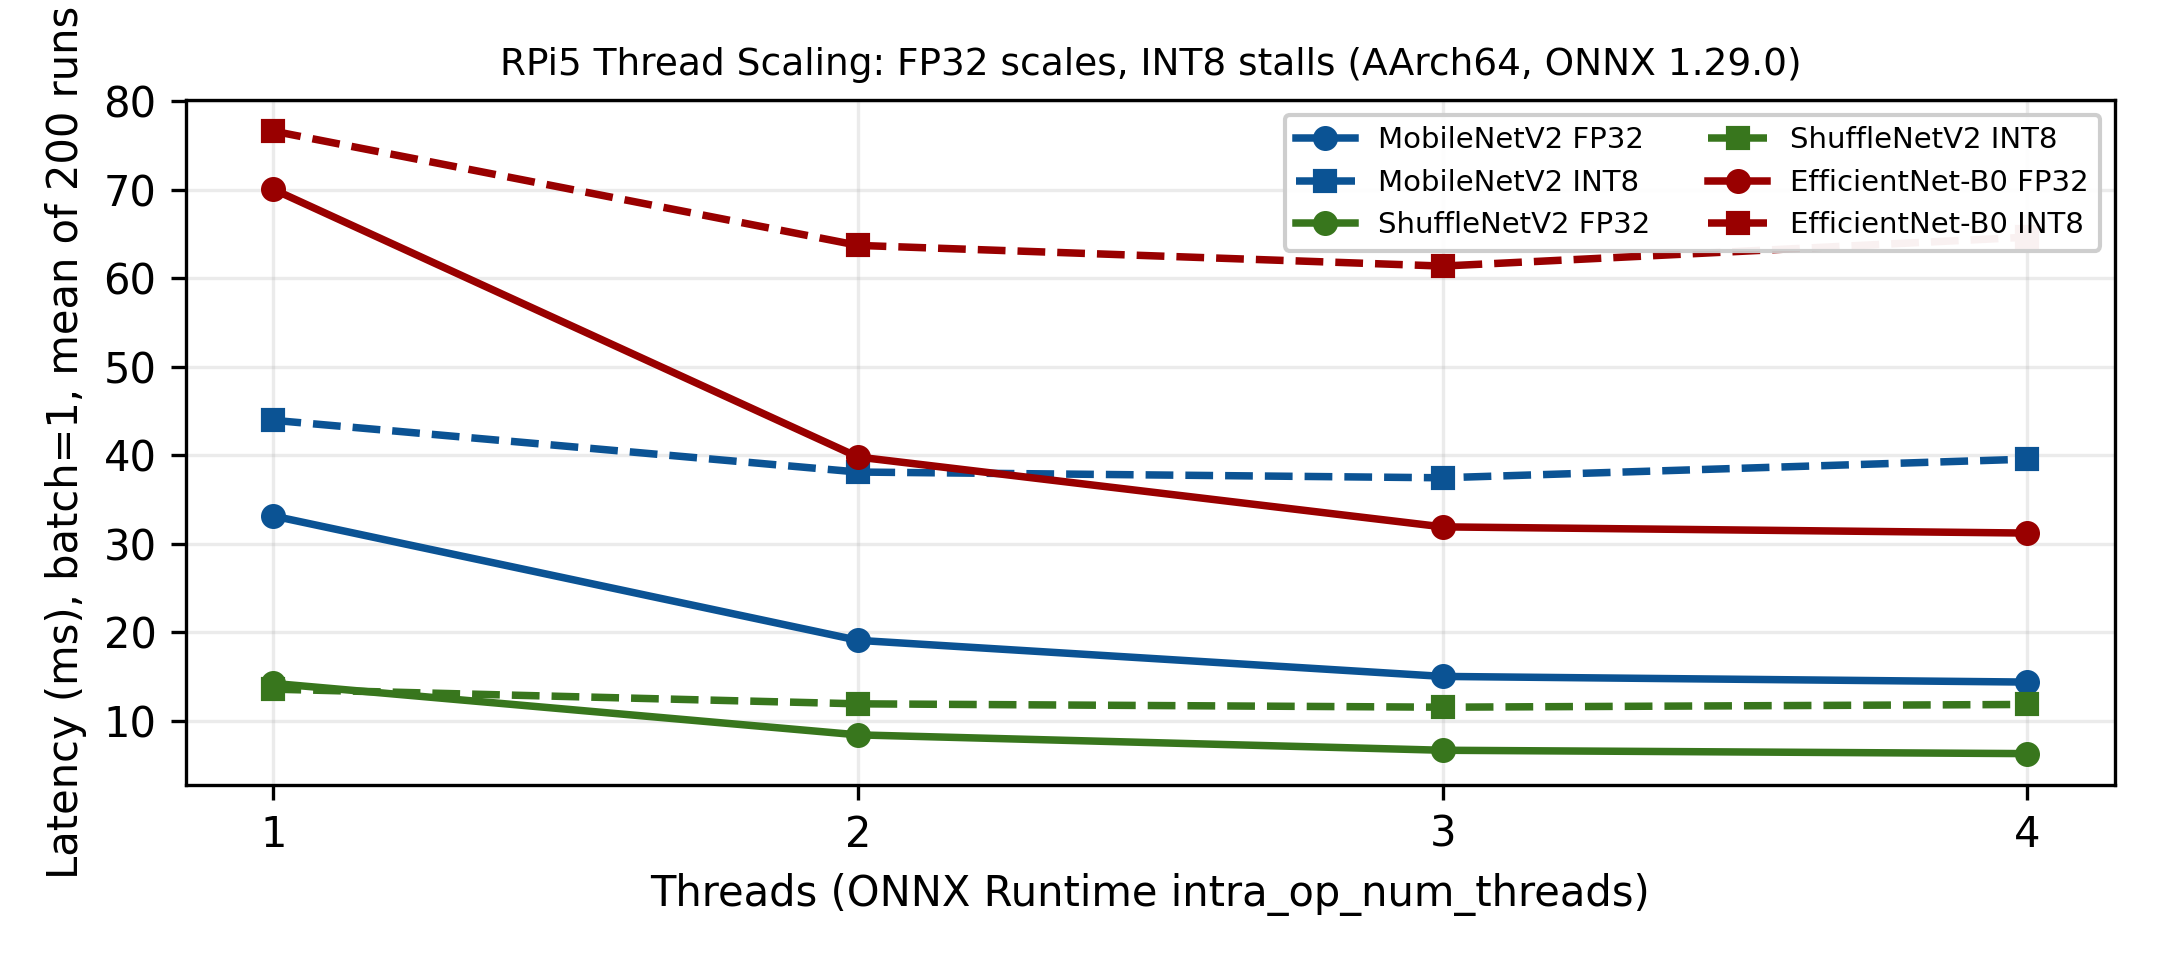
\includegraphics[width=0.95\linewidth]{rpi5_thread_scaling.png}
\caption{RPi5 thread scaling at batch=1. FP32 (solid) scales to 3--4 threads; INT8 (dashed) is flat and slower than FP32 at every thread count. The gap quantifies the dequantization bottleneck.}
\label{fig:rpi5thread}
\end{figure}

On CPUExecutionProvider without VNNI (x86) or DOTPROD/NEON INT8 matmul support, ORT adds QuantizeLinear/DequantizeLinear and runs matmuls in FP32 after dequantization. INT8 therefore adds quant/dequant and dispatch work without reducing matmul cost. Cost grows with the number of quantize boundaries: depthwise separable and SE blocks (MobileNetV2, EfficientNet-B0) create many small matmuls and slow down most (30.1$\times$ on x86, 2.76$\times$ on ARM), while homogeneous channel-shuffle blocks (ShuffleNetV2) slow down least (6.4$\times$ / 1.89$\times$). Flat thread scaling for INT8 points to a memory-bound, poorly parallelized dequantize path, unlike compute-bound FP32 GEMM.

\begin{figure}[htbp]
\centering
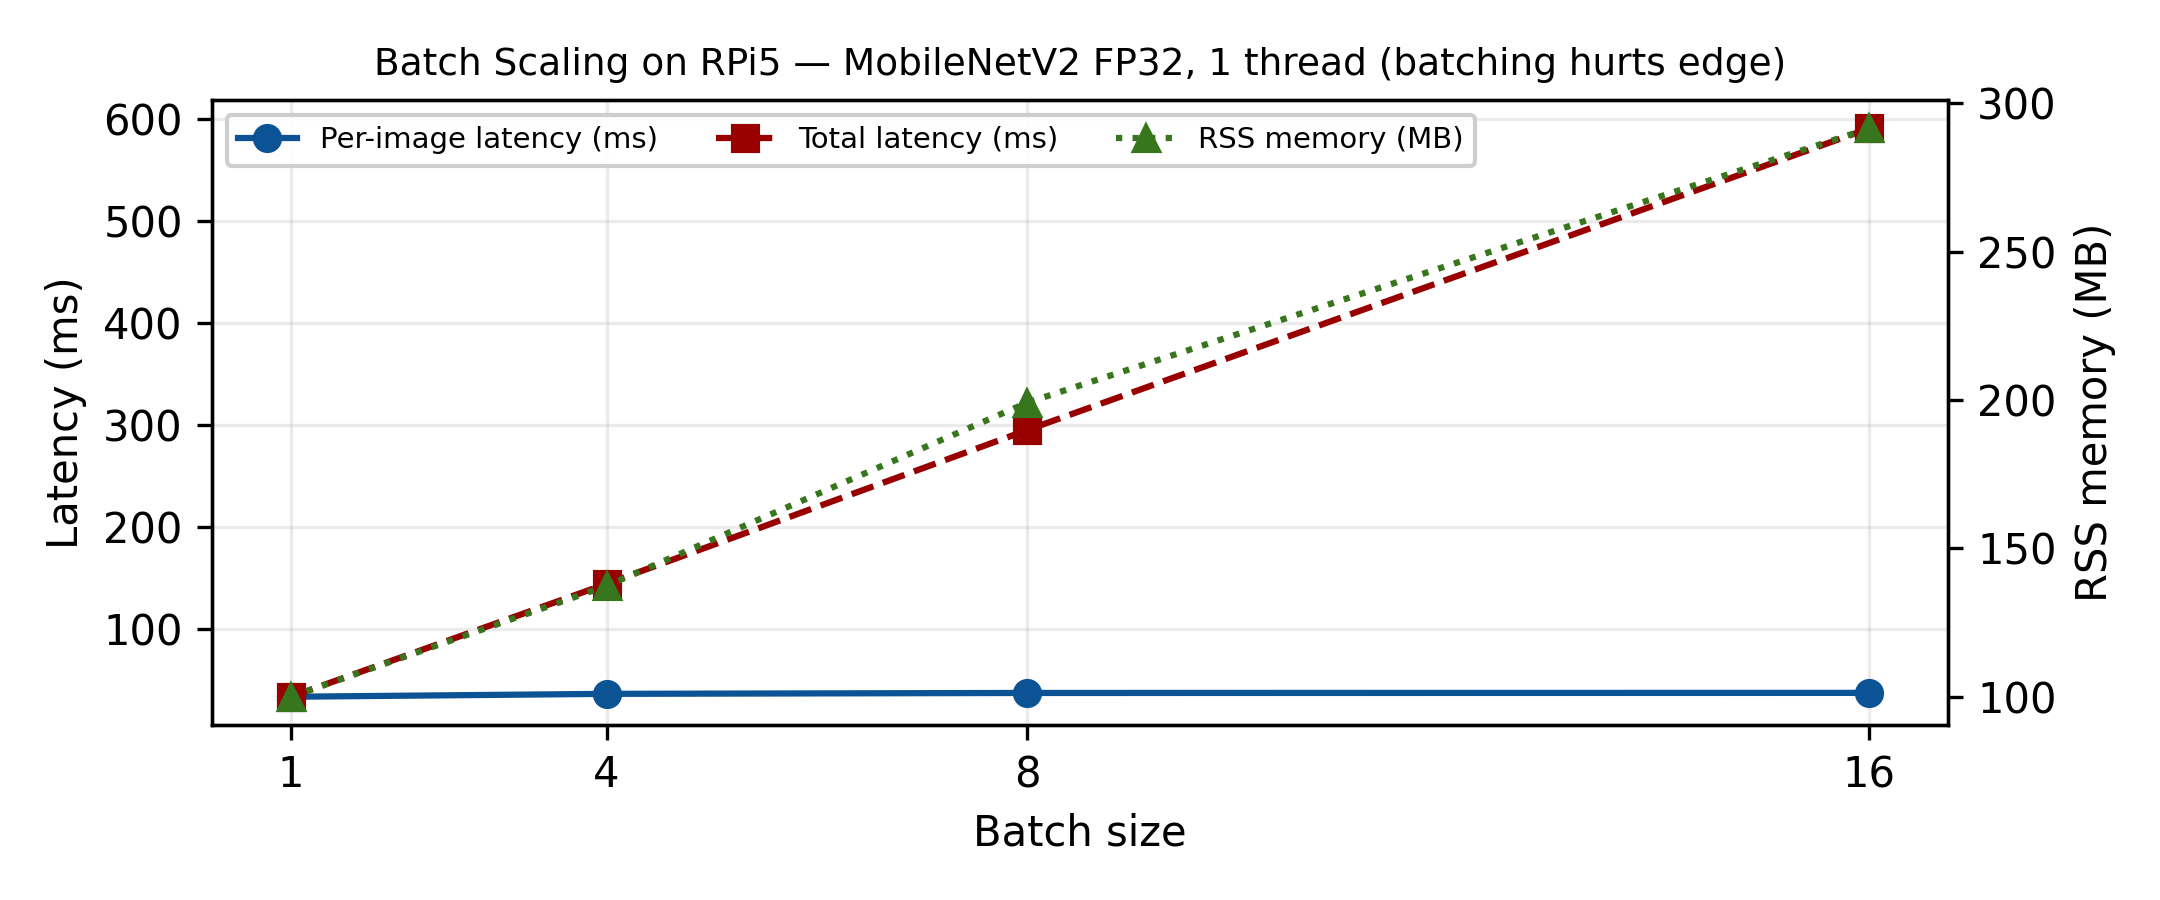
\includegraphics[width=0.95\linewidth]{rpi5_batch_scaling.png}
\caption{Batch scaling on RPi5 (MobileNetV2 FP32, 1 thread). Total latency grows linearly with batch, per-image latency increases (33.13\,ms at b=1 $\rightarrow$ 36.92\,ms at b=16), and RSS memory grows from 100\,MB to 292\,MB. For farm video streaming, batch=1 is optimal.}
\label{fig:rpi5batch}
\end{figure}

\textbf{Batch=1 is optimal for edge streaming.} Fig.~\ref{fig:rpi5batch} shows that batching hurts on RPi5: for MobileNetV2 FP32 at 1 thread, per-image latency rises from 33.13\,ms (b=1) to 35.98\,ms (b=4), 36.85\,ms (b=8), 36.92\,ms (b=16), while RSS grows from 100\,MB to 292\,MB. Total latency scales linearly (143.9\,ms at b=4, 294.8\,ms at b=8, 590.7\,ms at b=16). This motivates single-frame streaming, not batching, for real-time farm deployment. Model file size shrinks 3.3--3.7$\times$ with INT8 (e.g., 8.48$\rightarrow$2.30\,MB for MobileNetV2), but runtime RSS is dominated by the ORT arena and is similar across quantizations ($\sim$124\,MB for MobileNetV2), so INT8 does not save RAM at inference on this stack---a practical caveat for memory claims.

\begin{table}[htbp]
\caption{Level-2 Provenance: Node Expansion and ORT Kernel Quant Overhead (RPi5, 10 profiling runs, batch=1, 1 thread). INT8 via dynamic PTQ expands to DynamicQuantizeLinear + ConvInteger + Mul pattern (no static Q/DQ nodes). Overhead correlates with expansion and slowdown.}
\label{tab:level2}
\centering
\footnotesize
\setlength{\tabcolsep}{3.0pt}
\resizebox{\linewidth}{!}{\begin{tabular}{lcccccc}
\toprule
Model & FP32 nodes & INT8 nodes & Expansion & DynQuant/CvInt & Quant overhead & x86 / RPi5 slowdown \\
\midrule
MobileNetV2 & 170 & 487 & 2.86$\times$ & 53 / 52 & 29.2\% & 30.1$\times$ / 2.76$\times$ \\
ShuffleNetV2 & 902 & 1240 & 1.37$\times$ & 54 / 56 & 20.7\% & 6.4$\times$ / 1.89$\times$ \\
EfficientNet-B0 & 239 & 730 & 3.05$\times$ & 82 / 81 & 24.9\% & 23.0$\times$ / 2.07$\times$ \\
\bottomrule
\end{tabular}}
\end{table}

\textbf{Proven bottleneck (Level-2, measured).} Table~\ref{tab:level2} quantifies why INT8 is slower, beyond documentation claims. Dynamic PTQ does not insert static QuantizeLinear/DequantizeLinear nodes; it expands each Conv (52--81) into a DynamicQuantizeLinear + ConvInteger + Mul (scale) + Cast pattern, so node count grows by 1.37--3.05$\times$. ORT kernel profiling on RPi5 (batch=1, 1 thread, 10 runs) shows \texttt{Conv\_quant\_kernel} alone consumes 49.5--55.1\% of total time, and all quant-related kernels (QuantizeLinear, scale Mul, Cast, bias-add) add 20.7--29.2\% overhead, while the final \texttt{Gemm\_MatMul\_quant} is $<$0.1\%. The ranking matches the slowdown ranking: MobileNetV2 (29.2\% overhead, 2.86$\times$ expansion) suffers most, ShuffleNetV2 (20.7\%, 1.37$\times$) least. Artifact \texttt{results/profiling/level2\_profiling\_artifact.json} (shipped as supplementary) contains per-operator $\mu$s and full op counts, complementing TinyML system studies~\cite{david2021}.

\subsection{Accuracy--Latency--Size Trade-off}

\begin{figure}[htbp]
\centering

\includegraphics[width=0.95\linewidth]{pareto_frontier.png}
\caption{Accuracy--latency--size trade-off for the three architectures (circles: FP32; crosses: measured INT8). MobileNetV2-FP32 has the lowest x86 latency (1.85\,ms) at 97.83\% accuracy; EfficientNet-B0-FP32 has the highest accuracy (98.35\%) at 3.50\,ms. EfficientNet-B0-INT8 (35.46\% at 80.66\,ms) is off-scale and annotated. ShuffleNetV2-FP32 is strictly dominated by MobileNetV2-FP32 on accuracy--latency, so we report the dominated trade-off explicitly rather than a formal Pareto frontier.}
\label{fig:pareto}
\end{figure}

The trade-off (Fig.~\ref{fig:pareto}) shows that the best latency is MobileNetV2 FP32 at 1.85\,ms (541\,FPS) for real-time video, the smallest model is ShuffleNetV2 INT8 at 1.47\,MB for memory-constrained deployment, and the highest accuracy is EfficientNet-B0 FP32 at 98.35\% for veterinary diagnosis. The gap between best and worst FP32 accuracy is only 0.97\,pp (97.38\% versus 98.35\%); hardware constraints should drive model choice for deployment.

\subsection{Grad-CAM Interpretability}

\begin{figure}[htbp]
\centering
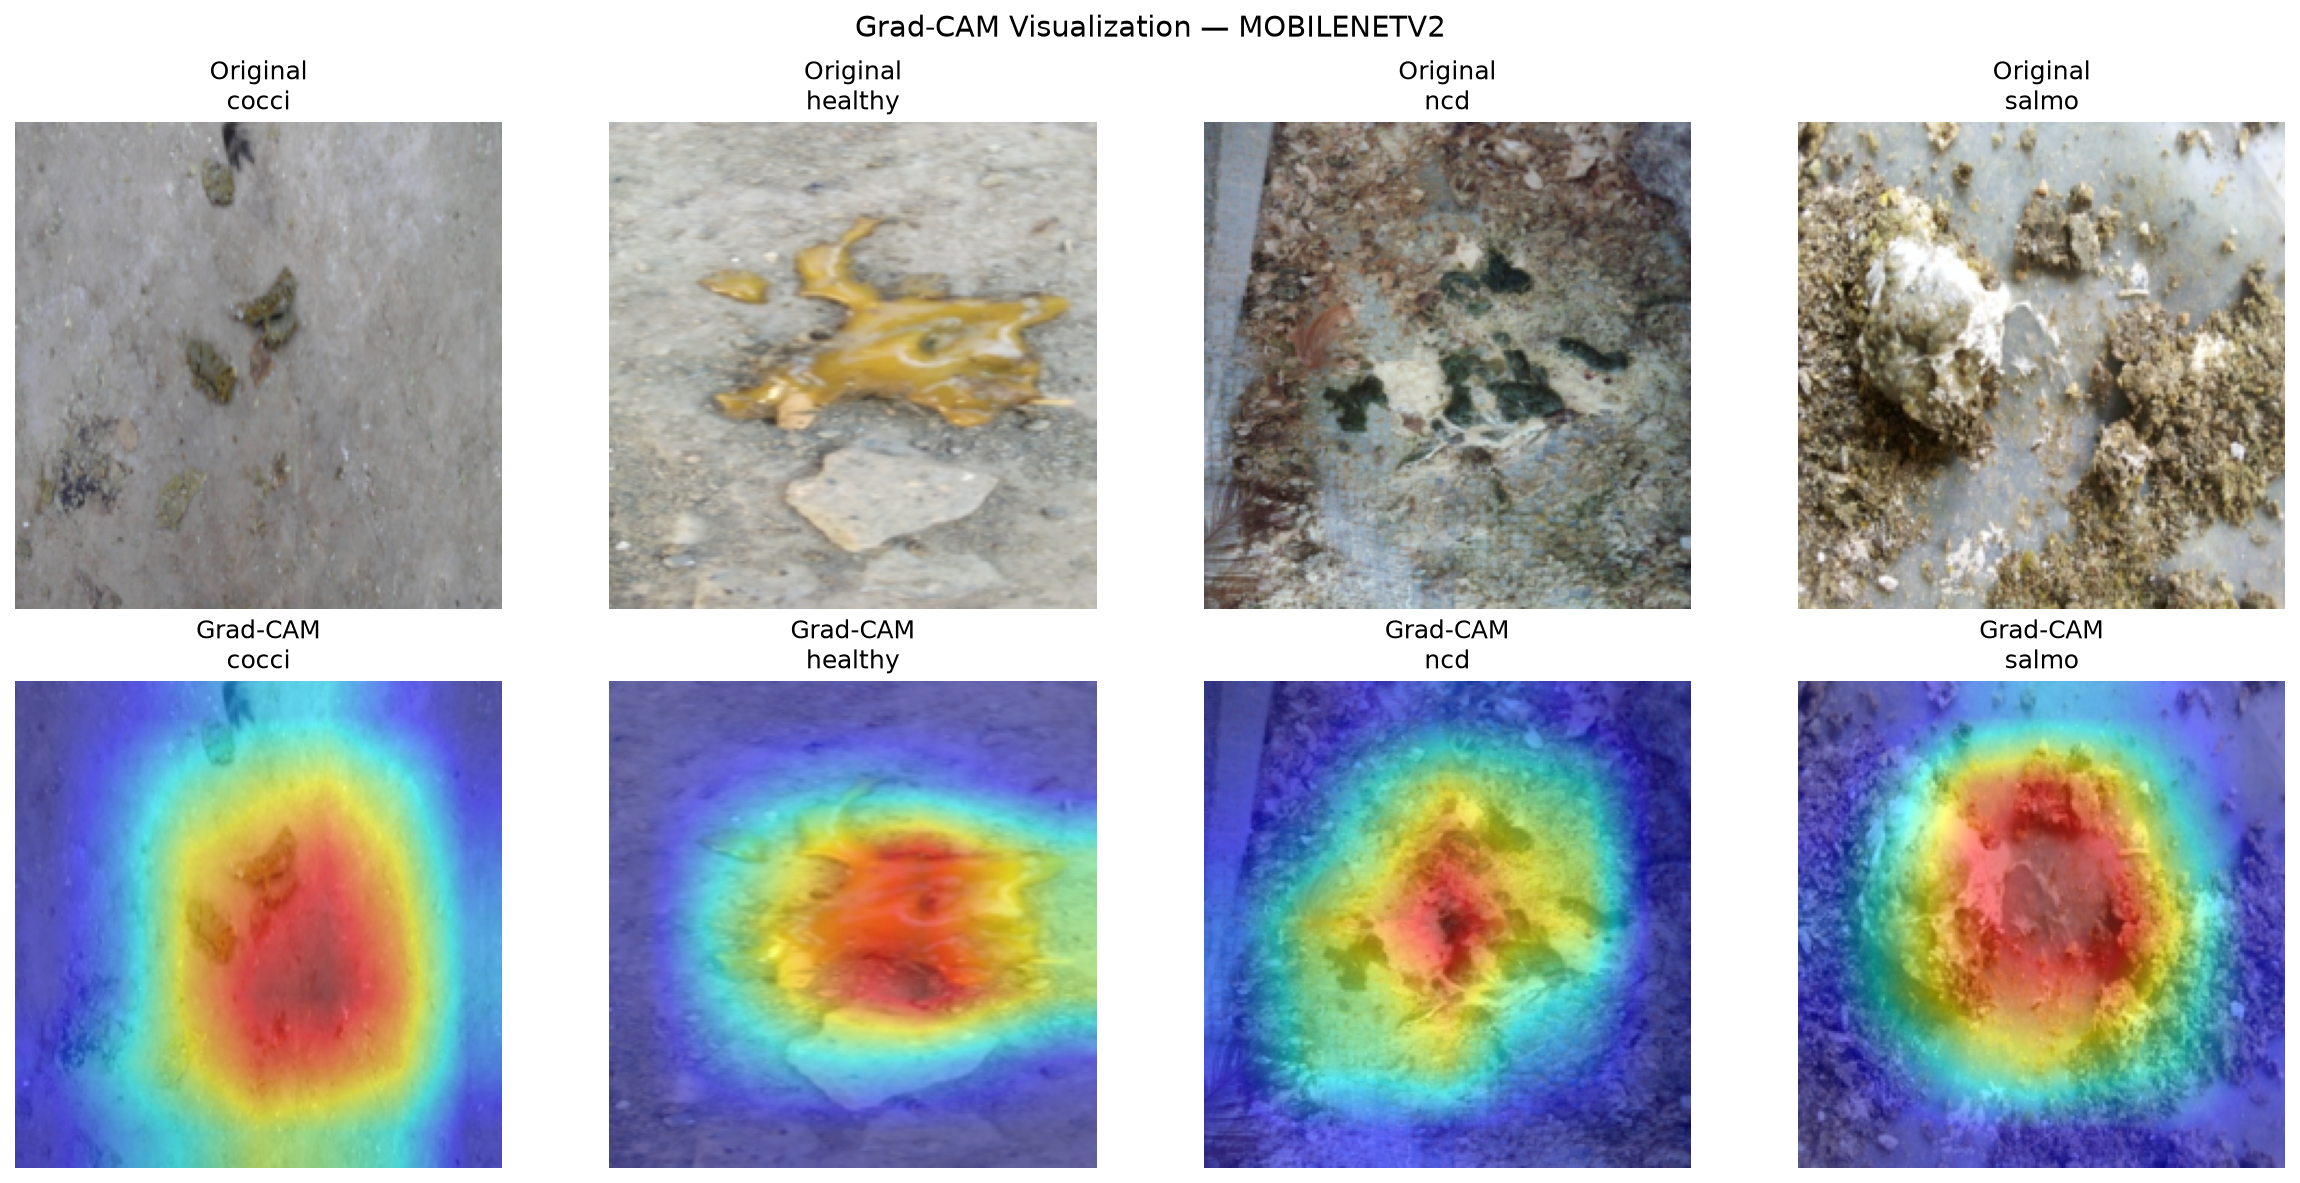
\includegraphics[width=0.95\linewidth]{gradcam_mobilenetv2.png}
\caption{Grad-CAM visualization for MobileNetV2 across the four classes (qualitative, single example per class). Heatmaps localize the fecal region rather than background; no quantitative attention metric is claimed.}
\label{fig:gradcam}
\end{figure}

Grad-CAM analysis~\cite{selvaraju2017} (Fig.~\ref{fig:gradcam}) provides a qualitative check that MobileNetV2 localizes the fecal region. Architecture-specific comparisons (EfficientNet-B0 SE attention, ShuffleNetV2 distributed attention) are visual observations from \texttt{figures/gradcam\_*.png}, not measured claims; a quantitative attention-overlap metric is future work.

\subsection{Comparison with Related Work}

\begin{table}[htbp]
\caption{Comparison with Existing Work}
\label{tab:comparison}
\centering
\begin{tabular}{lcccc}
\toprule
Work & Dataset & Best & Acc. & Edge \\
 & & Model & (\%) & Analysis \\
\midrule
Dhungana~\textit{et al.}~\cite{dhungana2025} & Machuve & EB0 & 99.1 & Web \\
Tasdelen~\textit{et al.}~\cite{tasdelen2025} & Machuve & MN2 & 97.1 & --- \\
Degu~\textit{et al.}~\cite{degu2023} & Machuve & R50 & 98.7 & Mobile \\
\textbf{Ours} & \textbf{Machuve/FecalFed} & \textbf{EB0} & \textbf{98.35} & \textbf{+INT8+trade-off} \\
\bottomrule
\end{tabular}
\end{table}

Our accuracy (98.35\%) is competitive with prior results on the same dataset family while providing additional analysis in quantization characterization, trade-off analysis, and interpretability that are absent from prior work.

\section{Conclusion}

This paper characterizes lightweight CNN architectures with INT8 quantization for poultry fecal disease detection. Our key findings are:

All three architectures exceed 97\% accuracy with ImageNet transfer learning, with EfficientNet-B0 at 98.35\%. INT8 PTQ increases latency by 6.4--30.1$\times$ on x86 and 1.9--2.8$\times$ on RPi5; on ARM, INT8 scales by only 1.1--1.2$\times$ from 1 to 4 threads versus 2.3$\times$ for FP32. ShuffleNetV2 degrades least (6.4$\times$ on x86, 1.89$\times$ on RPi5) due to its homogeneous design. INT8 accuracy is architecture-dependent (Table~\ref{tab:quantacc}): MobileNetV2 (+0.23\,pp) and ShuffleNetV2 (+0.06\,pp) are robust while EfficientNet-B0 collapses to 35.46\%. On RPi5, batch 1 is optimal and INT8 size reduction (3.3--3.7$\times$) does not reduce runtime RSS. The trade-off analysis identifies MobileNetV2 FP32 for latency-critical use (1.85\,ms on x86, 14.35\,ms on RPi5 at 4 threads) and ShuffleNetV2 INT8 for size-constrained use (1.47\,MB).

These findings enable practitioners to make informed deployment decisions based on their specific hardware constraints. This work characterized RPi5 deployment across 96 configurations; future work includes multi-seed variance reporting, QAT comparison (Maulana and Ramasamy report QAT outperforms PTQ), energy measurement on RPi5, and class imbalance mitigation for the underrepresented NCD class.

\begin{thebibliography}{99}

\bibitem{dhungana2025}
A.~Dhungana, X.~Yang, B.~Paneru, S.~Dahal, G.~Lu, and L.~Chai, ``An integrated deep learning approach for poultry disease detection and classification based on analysis of chicken manure images,'' \emph{AgriEngineering}, vol.~7, no.~9, p.~278, 2025. DOI: 10.3390/agriengineering7090278.

\bibitem{machuve2022}
D.~Machuve \textit{et al.}, ``Poultry diseases diagnostics models using deep learning,'' \emph{Frontiers in Artificial Intelligence}, vol.~5, p.~733345, 2022. DOI: 10.3389/frai.2022.733345.

\bibitem{tasdelen2025}
A.~Tasdelen and Y.~Arslan, ``Detection of high-risk diseases in poultry feces through transfer learning,'' \emph{Engineering Science and Technology, an International Journal}, vol.~64, p.~102002, 2025. DOI: 10.1016/j.jestch.2025.102002.

\bibitem{degu2023}
M.~Z.~Degu and G.~L.~Simegn, ``Smartphone based detection and classification of poultry diseases from chicken fecal images using deep learning techniques,'' \emph{Smart Agricultural Technology}, vol.~4, p.~100221, 2023. DOI: 10.1016/j.atech.2023.100221.

\bibitem{mobilenetv2}
M.~Sandler, A.~Howard, M.~Zhu, A.~Zhmoginov, and L.-C.~Chen, ``MobileNetV2: Inverted residuals and linear bottlenecks,'' in \emph{Proc. IEEE CVPR}, 2018, pp.~4510--4520.

\bibitem{shufflenetv2}
N.~Ma, X.~Zhang, H.-T.~Huang, and J.~Sun, ``ShuffleNetV2: Practical guidelines for efficient CNN architecture design,'' in \emph{Proc. ECCV}, 2018, pp.~116--131.

\bibitem{efficientnet}
M.~Tan and Q.~V.~Le, ``EfficientNet: Rethinking model scaling for convolutional neural networks,'' in \emph{Proc. ICML}, 2019, pp.~6105--6114.

\bibitem{jacob2018}
B.~Jacob \textit{et al.}, ``Quantization and training of neural networks for efficient integer-arithmetic-only inference,'' in \emph{Proc. IEEE CVPR}, 2018, pp.~2704--2713.

\bibitem{maulana2026}
D.~Maulana and R.~K.~Ramasamy, ``Systematic review of quantization-optimized lightweight transformer architectures for real-time fruit ripeness detection on edge devices,'' \emph{Computers}, vol.~15, no.~1, p.~69, 2026. DOI: 10.3390/computers15010069.

\bibitem{chi2026}
T.-Y.~Chi, ``FecalFed: Privacy-preserving poultry disease detection via federated learning,'' \textit{arXiv:2604.00559}, 2026. Dataset: HuggingFace \texttt{Dianyo/poultry-fecal-fl} (8,770 deduplicated images; accepted to the CVPR 2026 Workshop on Vision for Agriculture).

\bibitem{hoang2026}
T.-M.~Hoang \textit{et al.}, ``A comprehensive evaluation of lightweight deep learning models for tomato disease classification on edge computing environments,'' \emph{Scientific Reports}, vol.~16, p.~12320, 2026. DOI: 10.1038/s41598-026-42439-6.

\bibitem{onnxruntime2024}
Microsoft, ``Quantize ONNX models,'' ONNX Runtime Documentation, 2024. [Online]. Available: \url{https://onnxruntime.ai/docs/performance/quantization.html}

\bibitem{machuve22}
D.~Machuve \textit{et al.}, ``Machine learning dataset for poultry diseases diagnostics,'' Zenodo, 2022. DOI: 10.5281/zenodo.4628934.

\bibitem{nagel2021}
M.~Nagel \textit{et al.}, ``A white paper on neural network quantization,'' \textit{arXiv:2106.08295}, 2021.

\bibitem{selvaraju2017}
R.~R.~Selvaraju \textit{et al.}, ``Grad-CAM: Visual explanations from deep networks via gradient-based localization,'' in \emph{Proc. IEEE Int. Conf. Comput. Vis. (ICCV)}, 2017, pp.~618--626.

\bibitem{deng2009}
J.~Deng \textit{et al.}, ``ImageNet: A large-scale hierarchical image database,'' in \emph{Proc. IEEE Conf. Comput. Vis. Pattern Recognit. (CVPR)}, 2009, pp.~248--255.

\bibitem{david2021}
R.~David \textit{et al.}, ``TensorFlow Lite Micro: Embedded machine learning for TinyML systems,'' in \textit{Proc. Machine Learning and Systems (MLSys)}, 2021, pp.~800--815.

\end{thebibliography}

\end{document}
